
\begin{lemma}
The standard form of a conic is given by
\begin{align}
\frac{\vec{y}^{\top}D\vec{y}}{\vec{u}^{\top}\vec{V}^{-1}\vec{u}-f}&=1
\end{align}
\end{lemma}
Given
\begin{align}
\vec{x}^{\top}\myvec{\frac{1}{9} & 0 \\ 0 &\frac{-1}{16} }\vec{x}=1  
\end{align}
we have,
\begin{align}
    \vec{V} = \myvec{\frac{1}{9} & 0 \\ 0 &\frac{-1}{16} }
    \\
    \vec{u}^{\top}\vec{V}^{-1}\vec{u}-f = 1
    \\
    \vec{c} = -\vec{V}^{-1}\vec{u}=\myvec{0 \\ 0}
    \\
    \lambda_1 =  \frac{1}{9}, \lambda_2 = \frac{-1}{16}
\end{align}
Axes of hyperbola is given by
\begin{align}
    \sqrt{\frac{\vec{u}^{\top}\vec{V}^{-1}\vec{u}-f}{\lambda_1}} = 4\\ \sqrt{\frac{f-\vec{u}^{\top}\vec{V}^{-1}\vec{u}}{\lambda_2}} = 3
\end{align}
The vertices are given as
\begin{align}
    \pm\myvec{4 \\ 0}
\end{align}
Coordinates of foci are given by,
\begin{align}
  \vec{F} =\pm\brak{\sqrt{\frac{(\vec{u}^T\vec{V}^{-1}\vec{u}-f)(\lambda_2-\lambda_1)}{\lambda_1\lambda_2}}}\vec{p_1} \label{quadform/38/a/eq:1}
\end{align}
where, $\vec{p_1} = \myvec{1 \\ 0}$ since the equation of hyperbola is in standard form.
Substituting the values in \eqref{quadform/38/a/eq:1} we have,
\begin{align}
    \vec{F} = \pm\myvec{ 5 \\ 0}.
\end{align}
Eccentricity of the hyperbola is given by,
\begin{align}
   e = \frac{\sqrt{\frac{(\vec{u}^{\top}\vec{V}^{-1}\vec{u})(\lambda_2-\lambda_1)}{\lambda_1\lambda_2}}}{\sqrt{\frac{\vec{u}^{\top}\vec{V}^{-1}\vec{u}-f}{\lambda_1}}} \label{quadform/38/a/eq:2}
\end{align}
substituting the values in \eqref{quadform/38/a/eq:2},we have
\begin{align}
   e = \frac{5}{3}.
\end{align}
Length of the latus rectum is given by,
\begin{align}
    l = \frac{2\brak{{\sqrt{\frac{f-\vec{u}^{\top}\vec{V}^{-1}\vec{u}}{\lambda_2}}}}^2}{\sqrt{\frac{\vec{u}^{\top}\vec{V}^{-1}\vec{u}-f}{\lambda_1}}} \label{quadform/38/a/eq:3}
\end{align}
substituting the values in \eqref{quadform/38/a/eq:3},we have
\begin{align}
   l = \frac{32}{3}
\end{align}
Plot of the hyperbola:

\begin{figure}[!ht]
    \centering
    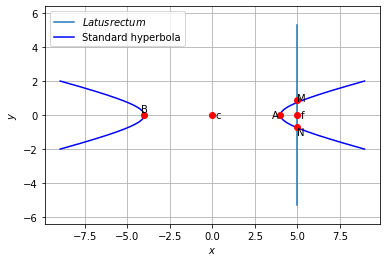
\includegraphics[width=\columnwidth]{solutions/su2021/2/38/a/hyperbola.png}
    \caption{Hyperbola}
    \label{quadform/38/a/fig:hyperbola}
\end{figure}  

